%%%%%%%%%%%%%%%%%%%%%%%%%%%%%%%%%%%%%%%%%
% Beamer Presentation - LaTeX Template
% Version 2.0 (March 8, 2022)
% Original Template: https://www.LaTeXTemplates.com
% Author: Vel (vel@latextemplates.com)
% License: CC BY-NC-SA 4.0

% Este modelo de apresentação foi
% criado a partir do modelo de Giovanni Spadaro.
% Disponível em: https://github.com/Giovo17/presentation-template-unict-lm-data
%
% Adaptado por Lucas Amaral Taylor para criar uma versão especial
% para os alunos de Matemática e Estatística da USP (IME-USP).
% Disponível em: https://github.com/lucasamtaylor01/IME-template
%%%%%%%%%%%%%%%%%%%%%%%%%%%%%%%%%%%%%%%%%

%----------------------------------------------------------------------------------------
% CLASSE DO DOCUMENTO E CONFIGURAÇÕES BÁSICAS
%----------------------------------------------------------------------------------------
\documentclass[
    % 11pt,
    presentation,               % Tamanho padrão da fonte
    % t,                % Alinhar verticalmente ao topo
    % aspectratio=169,   % Definir proporção 16:9
]{beamer}
\graphicspath{{img/}}         % Define o diretório das imagens

%----------------------------------------------------------------------------------------
% PACOTES NECESSÁRIOS
%----------------------------------------------------------------------------------------
\usepackage{
    booktabs,     % Melhora a aparência das linhas em tabelas
    palatino,     % Define Palatino como fonte principal
    subcaption    % Suporte para subfiguras
}
\usepackage{amsmath}
\usepackage{amssymb}
\usepackage{capt-of}
\usepackage{hyperref}
\usepackage{graphicx}
\usepackage{longtable}
\usepackage{wrapfig}
\usepackage{animate}
\usepackage{rotating}
\usepackage{bm}
\usepackage[normalem]{ulem}
\usepackage[T1]{fontenc} % Define Open Sans como fonte secundária
\usepackage[utf8]{inputenc}
\usepackage[font={small,it}]{caption}
\usepackage{tabulary}
\usepackage{tabularx}
\usepackage{color}
\usepackage{colortbl}
\usepackage{multirow}
\usepackage{tikz}
\usepackage{appendixnumberbeamer}
\usetikzlibrary{shadows}
\usetikzlibrary{patterns,intersections, positioning, decorations.markings}
\usetikzlibrary{patterns,decorations.pathreplacing,backgrounds,calc}
\usepackage{pgfplots}
\usepgfplotslibrary{fillbetween}
%----------------------------------------------------------------------------------------
%	PACOTES E CONFIGURAÇÕES PARA CÓDIGO
%----------------------------------------------------------------------------------------
% Pacotes necessários para formatação de código
\usepackage[utf8]{inputenc}
\usepackage{listings}
\usepackage{xcolor}

% Cores para syntax highlighting (VSCode Light Theme)
\definecolor{vscBackground}{RGB}{255,255,255}    % Fundo branco
\definecolor{vscKeyword}{RGB}{175,0,219}         % Roxo para palavras-chave
\definecolor{vscString}{RGB}{163,21,21}          % Vermelho para strings
\definecolor{vscComment}{RGB}{0,128,0}           % Verde para comentários
\definecolor{vscFunction}{RGB}{121,94,38}        % Marrom para funções
\definecolor{vscNumber}{RGB}{9,134,88}           % Verde escuro para números
\definecolor{vscOperator}{RGB}{175,0,219}        % Roxo para operadores
\definecolor{vscText}{RGB}{0,0,0}                % Texto preto
\definecolor{vscLineNr}{RGB}{128,128,128}        % Cinza para números de linha

% Configuração geral do listings para UTF-8
\lstset{
    inputencoding=utf8,
    extendedchars=true,
    literate=%
        {á}{{\'a}}1 {é}{{\'e}}1 {í}{{\'i}}1 {ó}{{\'o}}1 {ú}{{\'u}}1
        {Á}{{\'A}}1 {É}{{\'E}}1 {Í}{{\'I}}1 {Ó}{{\'O}}1 {Ú}{{\'U}}1
        {à}{{\`a}}1 {è}{{\`e}}1 {ì}{{\`i}}1 {ò}{{\`o}}1 {ù}{{\`u}}1
        {À}{{\`A}}1 {È}{{\'E}}1 {Ì}{{\`I}}1 {Ò}{{\`O}}1 {Ù}{{\`U}}1
        {ã}{{\~a}}1 {ẽ}{{\~e}}1 {ĩ}{{\~i}}1 {õ}{{\~o}}1 {ũ}{{\~u}}1
        {Ã}{{\~A}}1 {Ẽ}{{\~E}}1 {Ĩ}{{\~I}}1 {Õ}{{\~O}}1 {Ũ}{{\~U}}1
        {â}{{\^a}}1 {ê}{{\^e}}1 {î}{{\^i}}1 {ô}{{\^o}}1 {û}{{\^u}}1
        {Â}{{\^A}}1 {Ê}{{\^E}}1 {Î}{{\^I}}1 {Ô}{{\^O}}1 {Û}{{\^U}}1
        {ç}{{\c c}}1 {Ç}{{\c C}}1
        {º}{{\textordmasculine}}1
        {ª}{{\textordfeminine}}1
}

% Configurações base comum para todas as linguagens
\lstdefinestyle{baseStyle}{
    backgroundcolor=\color{vscBackground},
    basicstyle=\ttfamily\small\color{vscText},
    breakatwhitespace=false,
    breaklines=true,
    captionpos=b,
    keepspaces=true,
    numbers=left,
    numbersep=5pt,
    showspaces=false,
    showstringspaces=false,
    showtabs=false,
    tabsize=4,
    frame=single,
    framerule=0.8pt,
    rulecolor=\color{gray!20},
    numberstyle=\tiny\color{vscLineNr},
    keywordstyle=\color{vscKeyword},
    commentstyle=\color{vscComment}\itshape,
    stringstyle=\color{vscString},
    emphstyle=\color{vscFunction},
    columns=flexible,
    basewidth={0.5em,0.45em},
    inputencoding=utf8,
    extendedchars=true
}

%----------------------------------------------------------------------------------------
% Python
%----------------------------------------------------------------------------------------
\lstdefinestyle{pythonStyle}{
    style=baseStyle,
    language=Python,
    morekeywords={self,None,True,False,import,from,as,def,class,return,yield,
                  for,while,if,else,elif,try,except,finally,with,lambda,
                  async,await,break,continue,global,nonlocal,pass,raise},
    morekeywords=[2]{print,len,range,type,int,str,float,list,dict,set,
                     tuple,max,min,sum,sorted,enumerate,zip,map,filter,
                     any,all,abs,round,pow,divmod},
    keywordstyle=[2]\color{vscFunction},
    sensitive=true
}

\lstnewenvironment{python}[1][]{\lstset{style=pythonStyle, #1}}{}
\newcommand{\pyinline}[1]{\lstinline[style=pythonStyle]!#1!}
\newcommand{\inputpython}[2][]{\lstinputlisting[style=pythonStyle,#1]{#2}}

%----------------------------------------------------------------------------------------
% C Language
%----------------------------------------------------------------------------------------
\lstdefinestyle{cStyle}{
    style=baseStyle,
    language=C,
    morekeywords={include,define,void,int,char,float,double,long,unsigned,
                  struct,union,enum,typedef,const,static,extern,register,
                  auto,volatile,sizeof,return,if,else,for,while,do,switch,
                  case,break,continue,default,goto},
    morekeywords=[2]{printf,scanf,malloc,free,calloc,realloc,fopen,fclose,
                     fprintf,fscanf,strcpy,strlen,strcat},
    keywordstyle=[2]\color{vscFunction},
    sensitive=true
}

\lstnewenvironment{clang}[1][]{\lstset{style=cStyle, #1}}{}
\newcommand{\clinline}[1]{\lstinline[style=cStyle]!#1!}
\newcommand{\inputclang}[2][]{\lstinputlisting[style=cStyle,#1]{#2}}

%----------------------------------------------------------------------------------------
% C++
%----------------------------------------------------------------------------------------
\lstdefinestyle{cppStyle}{
    style=baseStyle,
    language=C++,
    morekeywords={class,private,protected,public,template,typename,namespace,
                  using,new,delete,this,friend,virtual,override,final,explicit,
                  mutable,constexpr,nullptr,noexcept,static_cast,dynamic_cast,
                  const_cast},
    morekeywords=[2]{cout,cin,endl,vector,string,map,set,queue,stack,pair,
                     begin,end,push_back,pop_back,emplace_back,size,empty},
    keywordstyle=[2]\color{vscFunction},
    sensitive=true
}

\lstnewenvironment{cpp}[1][]{\lstset{style=cppStyle, #1}}{}
\newcommand{\cppinline}[1]{\lstinline[style=cppStyle]!#1!}
\newcommand{\inputcpp}[2][]{\lstinputlisting[style=cppStyle,#1]{#2}}

%----------------------------------------------------------------------------------------
% R Language
%----------------------------------------------------------------------------------------
\lstdefinestyle{rStyle}{
    style=baseStyle,
    language=R,
    morekeywords={if,else,repeat,while,function,for,in,next,break,TRUE,FALSE,
                  NULL,Inf,NaN,NA,NA_integer_,NA_real_,NA_complex_,NA_character_},
    morekeywords=[2]{library,require,attach,detach,source,setwd,options,
                     data.frame,read.csv,write.csv,list,matrix,array},
    keywordstyle=[2]\color{vscFunction},
    sensitive=true
}

\lstnewenvironment{rlang}[1][]{\lstset{style=rStyle, #1}}{}
\newcommand{\rlinline}[1]{\lstinline[style=rStyle]!#1!}
\newcommand{\inputrlang}[2][]{\lstinputlisting[style=rStyle,#1]{#2}}

%----------------------------------------------------------------------------------------
% Java
%----------------------------------------------------------------------------------------
\lstdefinestyle{javaStyle}{
    style=baseStyle,
    language=Java,
    morekeywords={abstract,assert,boolean,break,byte,case,catch,char,class,
                  const,continue,default,do,double,else,enum,extends,final,
                  finally,float,for,if,implements,import,instanceof,int,
                  interface,long,native,new,package,private,protected,public,
                  return,short,static,strictfp,super,switch,synchronized,this,
                  throw,throws,transient,try,void,volatile,while},
    morekeywords=[2]{String,System,out,println,printStackTrace,ArrayList,
                     HashMap,Arrays,List,Map,Set,Exception,RuntimeException},
    keywordstyle=[2]\color{vscFunction},
    sensitive=true
}

\lstnewenvironment{java}[1][]{\lstset{style=javaStyle, #1}}{}
\newcommand{\javainline}[1]{\lstinline[style=javaStyle]!#1!}
\newcommand{\inputjava}[2][]{\lstinputlisting[style=javaStyle,#1]{#2}}       % Importa configurações para highlight de código

%----------------------------------------------------------------------------------------
% CONFIGURAÇÃO DO TEMA
%----------------------------------------------------------------------------------------
% Tema Base
\usetheme{CambridgeUS}                          % Define o tema principal
% \usetheme{Boadilla}                          % Define o tema principal
\useinnertheme{circles}                       % Tema interno com círculos
\useoutertheme[subsection=false]{miniframes}                   % Tema externo com miniframes
\setbeamertemplate{navigation symbols}{}     % Remove símbolos de navegação

% % Cores Personalizadas
\definecolor{primaryColor}{RGB}{157, 0, 0}   % Cor primária - azul escuro
\definecolor{secondaryColor}{RGB}{80, 0, 10} % Cor secundária - azul médio
\renewcommand{\vec}[1]{\bm{#1}}
\newcommand{\vinput}[1][x]{\vec{#1}}
\newcommand{\sample}[1][i]{\vec{s}_{#1}}
\newcommand{\adj}[1]{\boldsymbol{\mathtt{adj}}(#1)}
\newcommand{\rulesep}{\unskip\ \vrule\ }
\tikzset{
  invisible/.style={opacity=0},
  visible on/.style={alt={#1{}{invisible}}},
  alt/.code args={<#1>#2#3}{%
    \alt<#1>{\pgfkeysalso{#2}}{\pgfkeysalso{#3}} % \pgfkeysalso doesn't change the path
  },
}

\definecolor{mygray}{gray}{0.85}
\newcolumntype{g}{>{\columncolor{mygray}}c}

% % Configurações de Cores
% \setbeamertemplate{itemize item}{\color{primaryColor}}
\setbeamercolor{structure}{fg=primaryColor}
% \setbeamercolor{palette primary}{bg=primaryColor, fg=white}
% \setbeamercolor{palette secondary}{bg=secondaryColor, fg=white}
\setbeamercolor{title}{bg=primaryColor, fg=white}
\setbeamertemplate{caption}{\raggedright\insertcaption\par}
% % Cores do Cabeçalho e Rodapé
\setbeamercolor{headline}{bg=secondaryColor, fg=white}
% \setbeamercolor{section in head/foot}{bg=primaryColor, fg=white}
% \setbeamercolor{subsection in head/foot}{bg=secondaryColor, fg=white}
% \setbeamercolor{author in head/foot}{bg=primaryColor, fg=white}
% \setbeamercolor{title in head/foot}{bg=secondaryColor, fg=white}
% \setbeamercolor{date in head/foot}{bg=primaryColor, fg=white}
% \setbeamercolor{page number in head/foot}{bg=primaryColor, fg=white}
\setbeamerfont{caption}{size=\scriptsize}
%----------------------------------------------------------------------------------------
% BIBLIOGRAFIA
%----------------------------------------------------------------------------------------
\usepackage[style=alphabetic,backend=biber]{biblatex}
\addbibresource{bibliografia.bib}

%----------------------------------------------------------------------------------------
% INFORMAÇÕES DA APRESENTAÇÃO
%----------------------------------------------------------------------------------------
\title[$k$-NN Robustness Certification]{Exact Robustness Certification of $k$-Nearest Neighbor Classifiers}          % [Versão curta]{Versão completa}
\author{Ahmad Shakeel}            % [Versão curta]{Nome completo}
\institute[Univ. di Padova]{Master Degree in Computer Science \mbox{}\\ \mbox{}\\ Università degli Studi di Padova}
\date{10 Apr 2025}
\logo{

\includegraphics[scale=0.5, width=1cm]{img/unipd_logo}
}

%----------------------------------------------------------------------------------------
% INÍCIO DO DOCUMENTO
%----------------------------------------------------------------------------------------
\begin{document}

% Slide de título com logo
% \setbeamertemplate{headline}{}
% \setbeamertemplate{footline}{}
% \begin{frame}
%     \titlepage
%     \begin{figure}
%         \includegraphics[width=0.45\linewidth]{img/logo_IME.png}
%     \end{figure}
% \end{frame}

{
\defbeamertemplate*{headline}{mytheme}
{%
  \begin{beamercolorbox}[colsep=1.5pt]{upper separation line head}
  \end{beamercolorbox}
  \begin{beamercolorbox}{section in head/foot}
    \vskip2pt\phantom{\insertnavigation{\paperwidth}}\vskip2pt
  \end{beamercolorbox}%
  \begin{beamercolorbox}[colsep=1.5pt]{lower separation line head}
  \end{beamercolorbox}
}
  \setbeamertemplate{logo}{}
    \begin{frame}
        \titlepage
        \begin{figure}
            
\includegraphics[width=0.30\linewidth]{img/unipd_logo}
        \end{figure}
    \end{frame}
}

\begin{frame}{Outline}
    \tableofcontents
\end{frame}

\section{Introduction}

\begin{frame}{Adversarial Examples}

    \begin{alertblock}{Definition}
        Adversarial examples are carefully crafted input data designed to cause an AI system to produce incorrect or biased predictions (Szegedy et al., 2014).
    \end{alertblock}
    \begin{center}
        \begin{figure}
            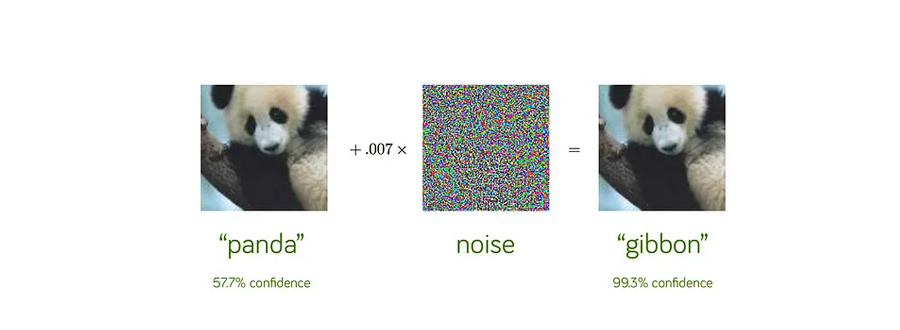
\includegraphics[width=0.70\linewidth]{img/AdvExample.png}
            \\ {\tiny Source: Szegedy et al. Explaining and harnessing adversarial examples}
        \end{figure}
    \end{center}

\end{frame}

\begin{frame}{Why do we care ?}

    \begin{itemize}
        \item Adversarial examples pose a significant security risks in safety-critical domains (e.g., healthcare, autonomous transportation, etc.)
        \begin{itemize}
            \item Compromised security systems;
            \item Data breaches and unauthorized access;
            \item Financial losses and fraud;
            \item \dots
        \end{itemize}
    \end{itemize}

\end{frame}

\begin{frame}[fragile]{$k$-NN}
    \begin{itemize}
        \item A \emph{non-parametric} supervised machine learning method;
        \item Suitable for both classification and regression tasks;
        \item Leverages data similarity to compute the prediction;
        \item Relies on distance metrics like Euclidean\\Manhattan or the general Minkowski distance;
    \end{itemize}

\end{frame}

\begin{frame}[fragile]{$3$-NN}
    \begin{figure}[H]
        \centering
        \usetikzlibrary{arrows.meta, intersections}
        \begin{tikzpicture}[
            dot/.style = {circle, draw, fill=#1, inner sep=3pt, node contents={}}
        ]
            \begin{axis}[
                xmin = 0, xmax = 6,
                ymin = 0, ymax = 6,
                xtick distance = 1,
                ytick distance = 1,
                grid = both,
                minor tick num = 5,
                major grid style = {lightgray},
                minor grid style = {lightgray!25},
                axis x line=center,
                axis y line=center,
                xlabel = {$x$},
                ylabel = {$y$},
                xlabel style={above left},
                ylabel style={below right}
            ]
            \node (x) at (3.5cm,3cm) [dot=gray!50];
            \node (l_x) at (3.5cm,3cm) {\textbf{\tiny x}};
			\node (c) at (3.5cm,3cm) [circle, draw, dashed, inner sep=0pt, minimum size=3cm, name path=C] {};
			\node (p1) at (2.5cm,5cm) [dot=green];
			\node (p2) at (4cm,4cm) [dot=green];
			\node (p3) at (5cm,1.5cm) [dot=green];
			\node (p4) at (1.5cm,4cm) [dot=green];
			\node (p5) at (1cm,2.5cm) [dot=blue!50];
			\node (p6) at (4cm,5.5cm) [dot=blue!50];
			\node (p6) at (5.5cm,4.5cm) [dot=blue!50];
			\node (p7) at (4cm,0.5cm) [dot=red];
			\node (p8) at (4.5cm,2.5cm) [dot=red];
			\node (p9) at (3cm,2cm) [dot=red];
			\node (p10) at (2.5cm,1cm) [dot=red];
			\draw [->] (x) -- (p2);
			\draw [->] (x) -- (p8);
			\draw [->] (x) -- (p9);
            \end{axis}
        \end{tikzpicture}
    \end{figure}
    \begin{center}
        \tiny 3NN over a dataset with 3 classes, which shows how a new  point is classified
    \end{center}
\end{frame}

\begin{frame}[fragile]{$3$-NN}
    \begin{figure}[H]
        \centering
        \usetikzlibrary{arrows.meta, intersections}
        \begin{tikzpicture}[
            dot/.style = {circle, draw, fill=#1, inner sep=3pt, node contents={}}
        ]
            \begin{axis}[
                xmin = 0, xmax = 6,
                ymin = 0, ymax = 6,
                xtick distance = 1,
                ytick distance = 1,
                grid = both,
                minor tick num = 5,
                major grid style = {lightgray},
                minor grid style = {lightgray!25},
                axis x line=center,
                axis y line=center,
                xlabel = {$x$},
                ylabel = {$y$},
                xlabel style={above left},
                ylabel style={below right}
            ]
            \node (m) at (3.5cm,3cm) [dot=red];
            \node (l_x) at (3.5cm,3cm) {\textbf{\tiny x}};
    		\node (p1) at (2.5cm,5cm) [dot=green];
			\node (p2) at (4cm,4cm) [dot=green];
			\node (p3) at (5cm,1.5cm) [dot=green];
			\node (p4) at (1.5cm,4cm) [dot=green];
			\node (p5) at (1cm,2.5cm) [dot=blue!50];
			\node (p6) at (4cm,5.5cm) [dot=blue!50];
			\node (p6) at (5.5cm,4.5cm) [dot=blue!50];
			\node (p7) at (4cm,0.5cm) [dot=red];
			\node (p8) at (4.5cm,2.5cm) [dot=red];
			\node (p9) at (3cm,2cm) [dot=red];
			\node (p10) at (2.5cm,1cm) [dot=red];
            \end{axis}
        \end{tikzpicture}
    \end{figure}
    \begin{center}
        \tiny 3NN over a dataset with 3 classes, which shows how a new  point is classified
    \end{center}
\end{frame}

\begin{frame}{Goal}

    \begin{itemize}
        \item Exact robustness certification of the $k$-Nearest Neighbors Classifier;
        \item Focus on \emph{completeness};
        \item Consider only the Euclidean distance as similarity metric.
    \end{itemize}
\end{frame}
\section{Methodology}
%----------------------------------------------------------------------------------------
\begin{frame}[fragile]{Robustness Certification: Basic idea}
    \begin{itemize}
        \item The possible perturbations of $x$ create a small $\ell_{\infty}$ ball centered in $x$ with radius $\epsilon > 0$:
            \[
                P^{\epsilon}(x) = \{x' \in \mathbb{R}^n\ |\ ||x'- x ||_{\infty} \leq \epsilon \}
            \]x
        \item $P^{\epsilon}(x)$ is called the \emph{Perturbation (or Adversarial)} region of $x$
    \end{itemize}
    \begin{figure}[H]
        \centering
        \usetikzlibrary{arrows.meta, intersections}
        \begin{tikzpicture}[
            scale=0.7,
            dot/.style = {circle, draw, fill=#1, inner sep=3pt, node contents={}}
        ]
            \begin{axis}[
                xmin = 0, xmax = 6,
                ymin = 0, ymax = 6,
                xtick distance = 1,
                ytick distance = 1,
                grid = both,
                minor tick num = 5,
                major grid style = {lightgray},
                minor grid style = {lightgray!25},
                axis x line=center,
                axis y line=center,
                xlabel = {$x$},
                ylabel = {$y$},
                xlabel style={above left},
                ylabel style={below right}
            ]
            \node (m) at (3.5cm,3cm) [dot=gray];
            \draw[fill=gray!70, draw=gray!70,semitransparent] (3cm,2.5cm) rectangle (4cm,3.5cm);
            \node (l_x) at (3.5cm,3cm) {\textbf{\tiny x}};
    		\node (p1) at (2.5cm,5cm) [dot=green];
			\node (p2) at (4cm,4cm) [dot=green];
			\node (p3) at (5cm,1.5cm) [dot=green];
			\node (p4) at (1.5cm,4cm) [dot=green];
			\node (p5) at (1cm,2.5cm) [dot=blue!50];
			\node (p6) at (4cm,5.5cm) [dot=blue!50];
			\node (p6) at (5.5cm,4.5cm) [dot=blue!50];
			\node (p7) at (4cm,0.5cm) [dot=red];
			\node (p8) at (4.5cm,2.5cm) [dot=red];
			\node (p9) at (3cm,2cm) [dot=red];
			\node (p10) at (2.5cm,1cm) [dot=red];
            \end{axis}
        \end{tikzpicture}
    \end{figure}
\end{frame}

\begin{frame}[fragile]{Robustness Certification: Stability}
    \begin{itemize}
        \item Check if exists $x_0 \in P^{\epsilon}(x)$ such that $k\text{-NN}(x) \neq k\text{-NN}(x_0)$
        \item $x_0$ exists $\Rightarrow $ $k$-NN is \textbf{not stable}  on $x$
        \item $x_0$ does not exist $\Rightarrow$ $k$-NN is \textbf{stable}  on $x$
    \end{itemize}
    \begin{figure}[H]
        \centering
        \usetikzlibrary{arrows.meta, intersections}
        \begin{tikzpicture}[
            scale=0.75,
            dot/.style = {circle, draw, fill=#1, inner sep=3pt, node contents={}}
        ]
            \begin{axis}[
                xmin = 0, xmax = 6,
                ymin = 0, ymax = 6,
                xtick distance = 1,
                ytick distance = 1,
                grid = both,
                minor tick num = 5,
                major grid style = {lightgray},
                minor grid style = {lightgray!25},
                axis x line=center,
                axis y line=center,
                xlabel = {$x$},
                ylabel = {$y$},
                xlabel style={above left},
                ylabel style={below right}
            ]
            \node (m) at (3.5cm,3cm) [dot=gray];
            \draw[fill=gray!70, draw=gray!70,semitransparent] (3cm,2.5cm) rectangle (4cm,3.5cm);
            \node (l_x) at (3.5cm,3cm) {\textbf{\tiny x}};

            \node (x_0) at (3.7cm,3.3cm) [black] {$\bullet$};
            \node [below right = -0.32cm and -0.32cm of x_0]{ $\scriptscriptstyle x_0$};
    		\node (p1) at (2.5cm,5cm) [dot=green];
			\node (p2) at (4cm,4cm) [dot=green];
			\node (p3) at (5cm,1.5cm) [dot=green];
			\node (p4) at (1.5cm,4cm) [dot=green];
			\node (p5) at (1cm,2.5cm) [dot=blue!50];
			\node (p6) at (4cm,5.5cm) [dot=blue!50];
			\node (p6) at (5.5cm,4.5cm) [dot=blue!50];
			\node (p7) at (4cm,0.5cm) [dot=red];
			\node (p8) at (4.5cm,2.5cm) [dot=red];
			\node (p9) at (3cm,2cm) [dot=red];
			\node (p10) at (2.5cm,1cm) [dot=red];
            \end{axis}
        \end{tikzpicture}
    \end{figure}
\end{frame}

\begin{frame}{Algorithm overview}
    Given an input samples $x$:
    \begin{enumerate}
        \item<2-> Build a directed graph $G$ where
            \begin{itemize}
                \item Nodes are samples in the training set;
                \item Edges model the relation of \textbf{\emph{being-closer}} to the adversarial region of $x$;
            \end{itemize}
        \item<3-> For each label $\ell$
            \begin{itemize}
                \item Traverse the graph $G$
                \item Find a \textbf{\emph{valid}} path with $k$ samples where $\ell$ is dominant label;
            \end{itemize}
         \item<4-> If more than one dominant label is found
            \begin{itemize}
                \item $k$-NN is not stable on $x$;
                \item otherwise $k$-NN is stable on $x$;
            \end{itemize}
    \end{enumerate}
\end{frame}

\begin{frame}[fragile]{Graph Construction}
    \begin{figure}[h]
        \centering
        \begin{subfigure}{0.5\linewidth}
            \begin{tikzpicture}[>=latex, scale=0.9]
                \centering
                \begin{axis}[
                    xmin = 0, xmax = 2,
                    ymin = 0, ymax = 2,
                    xtick distance = 1,
                    ytick distance = 1,
                    grid = both,
                    minor tick num = 10,
                    major grid style = {lightgray},
                    minor grid style = {lightgray!75},
                    width = 8cm,
                    height = 8cm,
                    axis x line=center,
                    axis y line=center,
                    xlabel = {$x$},
                    ylabel = {$y$},
                    xlabel style={above left},
                    ylabel style={below right}]

                        % draws point
                        \node [green, mark=*](x_2) at (1cm,1.8cm) {$\bullet$};
                        \node [below right = -0.32cm and -0.32cm of x_2]{ $\scriptscriptstyle \sample[2]$};
                        \node [green](x_1) at (2cm,1.6cm) {$\bullet$};
                        \node [below right = -0.32cm and -0.32cm of x_1]{$\scriptscriptstyle \sample[1]$};
                        \node [blue](x_3) at (3cm,1.8cm) {$\bullet$};
                        \node [below right = -0.25cm and -0.50cm of x_3]{$\scriptscriptstyle \sample[3]$};
                        \node [blue](x_4) at (3.2cm,1.8cm) {$\bullet$};
                        \node [below right = -0.60cm and -0.32cm of x_4]{$\scriptscriptstyle \sample[4]$};
                        \node [blue](x_5) at (3cm,3.4cm) {$\bullet$};
                        \node [below right = -0.32cm and -0.32cm of x_5]{$\scriptscriptstyle \sample[5]$};

                        \draw [dashed, visible on=<3-5>] (2cm, 0cm) -- (2cm, 10cm);
                        \draw [dashed, visible on=<6-7>] (3.1cm, 0cm) -- (3.1cm, 10cm);
                        \draw [dashed, visible on=<8-9>] (2.1cm, 0cm) -- (2.1cm, 10cm);

                        \draw[fill=gray!50, draw=gray!50,semitransparent] (1.75cm,1.75cm) rectangle (2.25cm,2.25cm);
                        \node [red](x) at (2cm,2cm) {$\bullet$};
                        \node [below right = -0.32cm and -0.32cm of x]{$\scriptscriptstyle \vinput$};

                        \end{axis}
            \end{tikzpicture}
        \end{subfigure}
        \begin{subfigure}{0.4\linewidth}
            \centering
            \begin{tikzpicture}[>=latex, scale=0.7, baseline={(2.7cm,1cm)}]

                \tikzset{% This is the style settings for nodes
                vertex/.style={circle,minimum size=1cm,fill=#1,draw,
                                        general shadow={fill=gray!60,shadow xshift=1pt,shadow yshift=-1pt}}}


                \node [vertex=green!25, visible on=<2->](s_1) at (3,10) {$\sample[1]$};
                \node [vertex=green!25, visible on=<2->](s_2) at (1,8) {$\sample[2]$};
                \node [vertex=blue!25, visible on=<2->](s_3) at (5,8) {$\sample[3]$};
                \node [vertex=blue!25, visible on=<2->](s_4) at (1,5) {$\sample[4]$};
                \node [vertex=blue!25, visible on=<2->](s_5) at (5,5) {$\sample[5]$};

                \draw [->,very thick, visible on=<10->] (s_1) -- (s_2);
                \draw [->,very thick, visible on=<10->] (s_1) -- (s_3);
                \draw [->,very thick, visible on=<10->] (s_1) to[bend right=70] (s_4);
                \draw [->,very thick, visible on=<10->] (s_1) to[bend left=70] (s_5);

                \draw [->,very thick, visible on=<4->] (s_2) to[bend right=10] (s_3);
                \draw [->,very thick, visible on=<9->] (s_2) to[bend right=10] (s_4);
                \draw [->,very thick, visible on=<11->](s_2) -- (s_5);

                \draw [->,very thick, visible on=<5->] (s_3) to[bend right=10] (s_2);
                \draw [->,very thick, visible on=<7->] (s_3) -- (s_4);
                \draw [->,very thick, visible on=<7->] (s_3) -- (s_4);
                \draw [->,very thick, visible on=<11->](s_3) -- (s_5);

                \draw [->,very thick, visible on=<9->] (s_4) to[bend right=10] (s_2);
                \draw [->,very thick, visible on=<11->] (s_4) -- (s_5);


            \end{tikzpicture}
        \end{subfigure}
    \end{figure}
\end{frame}


\begin{frame}<1-5>[fragile, label=graph-traversal]{Graph Traversal}
    \only<2-3>{$k=1$}
    \only<3>{--- Labels = $\{\textit{green}\}$}
    \only<3>{--- Stable = YES}
    \only<4-10>{$k=3$}
    \only<6-9>{--- Labels = $\{\textit{green}\}$}
    \only<10>{--- Labels = $\{\textit{green, blue}\}$}
    \only<10>{--- Stable = NO}
    % \only<11->{$k=5$}
    % \only<13>{--- Labels = $\{\textit{blue}\}$}
    % \only<13>{--- Stable = YES}
    \begin{figure}[h]
        \centering
        \begin{subfigure}{0.45\linewidth}
            \begin{tikzpicture}[>=latex, scale=0.7, baseline={(-1cm,-1cm)}]

                \tikzset{% This is the style settings for nodes
                    yshift=-1.5cm,
                    xshift=-1.5cm,
                    vertex/.style={circle,minimum size=0.5cm,fill=#1,draw,
                                        general shadow={fill=gray!60,shadow xshift=1pt,shadow yshift=-1pt}}}


                    \node [vertex=green!25](s_1) at (1,8) {$\sample[1]$};
                    \node [vertex=green!25](s_2) at (-1,6) {$\sample[2]$};
                    \node [vertex=blue!25](s_3) at (3,6) {$\sample[3]$};
                    \node [vertex=blue!25](s_4) at (-1,3) {$\sample[4]$};
                    \node [vertex=blue!25](s_5) at (3,3) {$\sample[5]$};

                    \draw [->,very thick] (s_1) -- (s_2);
                    \draw [->,very thick] (s_1) -- (s_3);
                    \draw [->,very thick] (s_1) to[bend right=70] (s_4);
                    \draw [->,very thick] (s_1) to[bend left=70] (s_5);

                    \draw [->,very thick] (s_2) to[bend right=10] (s_3);
                    \draw [->,very thick] (s_2) to[bend right=10] (s_4);
                    \draw [->,very thick](s_2) -- (s_5);

                    \draw [->,very thick] (s_3) to[bend right=10] (s_2);
                    \draw [->,very thick] (s_3) -- (s_4);
                    \draw [->,very thick] (s_3) -- (s_4);
                    \draw [->,very thick](s_3) -- (s_5);

                    \draw [->,very thick] (s_4) to[bend right=10] (s_2);
                    \draw [->,very thick] (s_4) -- (s_5);

            \end{tikzpicture}
        \end{subfigure}
        \onslide<2->{\rulesep}
        \begin{subfigure}{0.4\linewidth}
            \centering
            \begin{tikzpicture}[>=latex, scale=0.7, baseline={(2.7cm,1cm)}]

                \tikzset{% This is the style settings for nodes
                vertex/.style={circle,minimum size=0.5cm,fill=#1,draw,
                                        general shadow={fill=gray!60,shadow xshift=1pt,shadow yshift=-1pt}},
                cross/.style={
                    decoration={markings, mark=at position 0.5 with {
                        \node[scale=1.5, inner sep=0pt] {$\times$};
                    }},
                    postaction={decorate}
                }}

                \node [vertex=green!25, visible on=<2->](s_1) at (3,10) {$\sample[1]$};
                \node [vertex=green!25, visible on=<5-10>](s_12) at (1,8.5) {$\sample[2]$};
                \node [vertex=blue!25, visible on=<5-10>](s_123) at (1,6.5) {$\sample[3]$};
                \node [vertex=blue!25, visible on=<7-8>](s_124) at (3,6.5) {$\sample[4]$};
                \node [vertex=blue!25, visible on=<9-10>](s_13) at (3,8) {$\sample[3]$};
                \node [vertex=blue!25, visible on=<9-10>](s_134) at (3,6) {$\sample[4]$};
                % \node [vertex=green!25, visible on=<12->](s_12_) at (3,8) {$\sample[2]$};
                % \node [vertex=blue!25, visible on=<12->](s_123_) at (3,6) {$\sample[3]$};
                % \node [vertex=blue!25, visible on=<12->](s_1234_) at (3,4) {$\sample[4]$};
                % \node [vertex=blue!25, visible on=<12->](s_12345_) at (3,2) {$\sample[5]$};

                \draw [->,very thick, visible on=<5-10>] (s_1) -- (s_12);
                \draw [->,very thick, visible on=<5-10>] (s_12) -- (s_123);
                \draw [->,very thick, visible on=<7>] (s_12) -- (s_124);
                \draw [cross, ->,very thick, visible on=<8>] (s_12) -- (s_124);
                \draw [->,very thick, visible on=<9-10>] (s_1) -- (s_13);
                \draw [->,very thick, visible on=<9-10>] (s_13) -- (s_134);
                % \draw [->,very thick, visible on=<12->] (s_1) -- (s_12_);
                % \draw [->,very thick, visible on=<12->] (s_12_) -- (s_123_);
                % \draw [->,very thick, visible on=<12->] (s_123_) -- (s_1234_);
                % \draw [->,very thick, visible on=<12->] (s_1234_) -- (s_12345_);

            \end{tikzpicture}
        \end{subfigure}
    \end{figure}
\end{frame}

\begin{frame}<1>[fragile, label=validity-region]{Graph Construction}
    \begin{figure}[h]
        \centering
        \begin{tikzpicture}[>=latex, scale=0.9]
            \centering
            \begin{axis}[
                xmin = 0, xmax = 2,
                ymin = 0, ymax = 2,
                xtick distance = 1,
                ytick distance = 1,
                grid = both,
                minor tick num = 10,
                major grid style = {lightgray},
                minor grid style = {lightgray!75},
                width = 8cm,
                height = 8cm,
                axis x line=center,
                axis y line=center,
                xlabel = {$x$},
                ylabel = {$y$},
                xlabel style={above left},
                ylabel style={below right}]

                    % draws point
                    \node [green, mark=*](x_2) at (1cm,1.8cm) {$\bullet$};
                    \node [below right = -0.32cm and -0.32cm of x_2]{ $\scriptscriptstyle \sample[2]$};
                    \node [green](x_1) at (2cm,1.6cm) {$\bullet$};
                    \node [below right = -0.32cm and -0.32cm of x_1]{$\scriptscriptstyle \sample[1]$};
                    \node [blue](x_3) at (3cm,1.8cm) {$\bullet$};
                    \node [below right = -0.25cm and -0.50cm of x_3]{$\scriptscriptstyle \sample[3]$};
                    \node [blue](x_4) at (3.2cm,1.8cm) {$\bullet$};
                    \node [below right = -0.60cm and -0.32cm of x_4]{$\scriptscriptstyle \sample[4]$};
                    \node [blue](x_5) at (3cm,3.4cm) {$\bullet$};
                    \node [below right = -0.32cm and -0.32cm of x_5]{$\scriptscriptstyle \sample[5]$};

                    \draw[fill=green, draw=green!50,semitransparent, visible on=<1>] (1.75cm,1.75cm) rectangle (2.1cm,2.25cm);
                    \draw[fill=blue, draw=blue!50,semitransparent, visible on=<2>] (2.1cm,1.75cm) rectangle (2.25cm,2.25cm);
                    % \draw[fill=blue, draw=blue!50,semitransparent, visible on=<3>] (1.75cm,1.75cm) rectangle (2.1cm,2.25cm);


                    \draw[fill=gray!50, draw=gray!50,semitransparent] (1.75cm,1.75cm) rectangle (2.25cm,2.25cm);
                    \node [red](x) at (2cm,2cm) {$\bullet$};
                    \node [below right = -0.32cm and -0.32cm of x]{$\scriptscriptstyle \vinput$};

                    \end{axis}
        \end{tikzpicture}
    \end{figure}
\end{frame}

\againframe<6-9>{graph-traversal}
\againframe<2>{validity-region}
\againframe<10>{graph-traversal}
% \againframe<10-12>{graph-traversal}
% \againframe<3>{validity-region}
% \againframe<13->{graph-traversal}


\begin{frame}{Graph Traversal-Summary}

    \begin{itemize}
        \item Start traversal of the graph from sample $\sample[i]$ not dominated by any other samples;

        \item Consider only the paths $[\sample[1], \sample[2], \ldots, \sample[k]]$ such that
            $\sample[1], \sample[2], \ldots, \sample[k]$ are the closest samples to some $x' \in P^{\epsilon}(\vinput)$ than any other samples;
    \end{itemize}
\end{frame}



\section{Experimental Evaluation}

\begin{frame}{Experimental Evaluation}
    \begin{itemize}
        \item Evaluated $k$-NN robustness  using 7 datasets;
        \item Used $k \in \{1,3,5,7\}$;
        \item Perturbation region with $\epsilon$ up to $0.05$;
    \end{itemize}
\end{frame}

% \begin{frame}{Evaluation Metrics}
%     Evaluated $k$-NN on the following metrics:
%     \begin{itemize}
%         \item \textbf{Robustness}: $k$-NN stable on $x$ and correct
%             \[
%                 \forall x_0 \in P^{\epsilon}(x)\quad k\text{-NN}(x_0)= \text{ ground truth of } x
%             \]
%         \item \textbf{Individual Fairness}: Similar individual should be treated similarly
%             \[
%                 \forall x, x_0 \in \mathbb{R}^n\quad \delta(x, x_0) \leq \epsilon \Rightarrow  k\text{-NN}(x)= k\text{-NN}(x_0)
%             \]
%     \end{itemize}
% \end{frame}

\begin{frame}[shrink=5]{Datasets}
    \begin{table}[H]
        \small
        \begin{tabular}{|l|g|g|g|g|g|}
            \hline
            \rowcolor{white}
            \textbf{Name} & \#training & \#test & \#features & \#features (one-hot) & \#classes \\
            \hline\hline
            \rowcolor{white}
            Australian    &   483 &  207  &  14 &  39 &  2 \\
            BreastCancer  &   479 &  204  &  10 &  10 &  2 \\
            \rowcolor{white}
            Diabetes      &   556 &  230  &   8 &   8 &  2 \\
            Fourclass     &   604 &  258  &   2 &   2 &  2 \\
            \rowcolor{white}
            Letter        & 15000 & 5000  &  16 &  16 & 26 \\
            Pendigits     &  7494 & 3498  &  16 &  16 & 10 \\
            \rowcolor{white}
            Satimage      &  4435 & 2000  &  36 &  36 &  6 \\
            \hline
        \end{tabular}
    \end{table}
\end{frame}

\begin{frame}{Preprocessing}
    \begin{itemize}
        \item Rows and columns with missing values are dropped;
        \item When needed, datasets are split into training ($\approx 70-80\%$) and test ($\approx 20-30\%$) sets;
        \item Categorical features are one-hot encoded;
        \item Numerical features are scaled to $[0,1]$ range.
    \end{itemize}
\end{frame}

\begin{frame}[fragile, shrink=5]{Robustness Results}
    \begin{figure}[H]
        \centering
        \pgfplotstableread{
            epsilon k1 k3 k5 k7
            0.1 97.6 97.6 97.4 97.4
            0.2 97.5 97.5 97.3 97.3
            0.5 97.2 97.2 97.0 97.0
            1 96.4 96.6 96.4 96.3
            2 94.4 94.5 94.5 94.2
            3 91.2 91.6 91.7 91.8
            4 86.2 88.5 88.9 89.0
        }\loadedtable
        \pgfplotsset{grid style={dashed}}
        \begin{tikzpicture}
            \begin{axis}[
                title = {\small \bfseries Pendigits},
                xlabel = {\footnotesize Perturbation (\%)},
                ylabel = {\footnotesize Certified Robustness (\%)},
                xtick={0,1,2,3,4},
                ytick={80,85,90,95,100},
                width = 6cm,
                height = 6cm,
                grid = both,
                major grid style = {lightgray},
                legend style = {nodes={scale=0.7, transform shape}},
                legend pos = north east,
                legend entries = {$k = 1$, $k = 3$, $k = 5$, $k = 7$},
                no markers,
                every axis plot/.append style = {thick}
                ]
                \addplot table [x=epsilon,y=k1] {\loadedtable};
                \addplot table [x=epsilon,y=k3] {\loadedtable};
                \addplot table [x=epsilon,y=k5] {\loadedtable};
                \addplot table [x=epsilon,y=k7] {\loadedtable};
            \end{axis}
        \end{tikzpicture}
        \quad
            \pgfplotstableread{
            epsilon k1 k3 k5 k7
            0.1 70.0 71.7 69.6 71.3
            0.2 68.6 70.0 68.2 71.3
            0.5 63.9 67.3 67.3 67.8
            1 58.6 63.0 63.0 61.7
            2 45.6 47.8 50.0 54.4
            3 33.4 37.3 41.3 44.7
            4 27.3 29.5 33.4 38.2
        }\loadedtable
        \pgfplotsset{grid style={dashed}}
        \begin{tikzpicture}
            \begin{axis}[
                title = {\small \bfseries Diabetes},
                xlabel = {\footnotesize Perturbation (\%)},
                ylabel = {\footnotesize Certified Robustness (\%)},
                xtick={0,1,2,3,4},
                ytick={30,40,50,60,70},
                width = 6cm,
                height = 6cm,
                grid = both,
                major grid style = {lightgray},
                legend style = {nodes={scale=0.7, transform shape}},
                legend pos = north east,
                legend entries = {$k = 1$, $k = 3$, $k = 5$, $k = 7$},
                no markers,
                every axis plot/.append style = {thick}
                ]
                \addplot table [x=epsilon,y=k1] {\loadedtable};
                \addplot table [x=epsilon,y=k3] {\loadedtable};
                \addplot table [x=epsilon,y=k5] {\loadedtable};
                \addplot table [x=epsilon,y=k7] {\loadedtable};
            \end{axis}
            \end{tikzpicture}
    \end{figure}
\end{frame}

\begin{frame}{Limitations}
    \begin{itemize}
        \item Not always able to scale over high value of $k$ or $\epsilon$;
        \item Much time wasted on finding a path which does not exist;
    \end{itemize}
    \begin{table}[H]
        \centering
     \begin{tabular}{|l|g|g|g|}
            \hline
            \rowcolor{white}
            \textbf{Name} & $\epsilon$& Avg.\ Time per $\epsilon$ (seconds) \\
            \hline\hline
            \rowcolor{white}
            Australian   & [0.001, 0.05] & 2 \\
            BreastCancer & [0.001, 0.05] & 2.75\\
            \rowcolor{white}
            Diabetes      & [0.001, 0.04] & 180  \\
            Fourclass     & [0.001, 0.04] & 1.2 \\
            \rowcolor{white}
            Letter        & [0.001, 0.01] & 120 \\
            Pendigits     & [0.001, 0.04] & 900 \\
            \rowcolor{white}
            Satimage      & [0.001, 0.01] & 120 \\
            \hline
        \end{tabular}
    \end{table}
\end{frame}
\section{Conclusion and Future work}

\begin{frame}{Conclusion}
  \begin{itemize}
    \item Developed a novel algorithm to certify the robustness of $k$-NN;
    \item Focus on completeness;
    \item Experimental evaluation showed overall good results;
  \end{itemize}
\end{frame}

\begin{frame}{Future Works}
  \begin{itemize}
    \item Leverage high-order voronoi diagram to further reduce certification time;
    \item Adapt the algorithm to other distance metrics like the Manhattan distance or the more general
          Minkoswki distance.
  \end{itemize}
\end{frame}




\begin{frame}
  \centering
  \centering \Large \emph{Thanks for listening !!}
\end{frame}

\appendix

\begin{frame}{Graph Construction Optimization}

  Consider only the samples within the hyperball centered in $x$ and radius
               \[
                     2\epsilon\sqrt{N} + d
               \]
  where \begin{itemize}
     \item $\epsilon$ is the radius of the $\ell_{\infty}$ ball;
     \item $d$ the distance between $x$ and its $k$-th closest sample;
     \item $N$ is the number of features;
  \end{itemize}
  \begin{alertblock}{Proposition}
     Given a perturbation region $P^{\epsilon}(x)$, the hyperball centered in $x$ with radius $2\epsilon\sqrt{N} + d$
     contains the $k$ closest samples of every point $x_0 \in P^{\epsilon}(x)$
  \end{alertblock}
 \end{frame}


% \include{sections/section02}
% \include{sections/section03}

% % Slide final
% \begin{frame}
%     \begin{center}
%         {\Huge Fim da apresentação!}
%     \end{center}
% \end{frame}

\end{document}


